\documentclass[12pt,a4paper]{article}

% ---------------- Packages ----------------
\usepackage[utf8]{inputenc}
\usepackage{amsmath, amssymb, amsthm}
\usepackage{graphicx}
\usepackage{hyperref}
\usepackage{geometry}
\usepackage[ style=authoryear,maxcitenames=2,maxbibnames=99]{biblatex}
\addbibresource{refer.bib} % your .bib file
\setlength\bibitemsep{1.2\baselineskip}
\usepackage{url}
\usepackage{hyperref}
\sloppy  % allows looser line breaks
\emergencystretch=2em

\DeclareUnicodeCharacter{2061}{}

\geometry{margin=1in}

% ---------------- Title Info ----------------
\title{ AuON: A Survey For Linear-time Orthogonal Optimizer }
\author{Dipan Maity \\
\texttt{dipanai.xyz@gmail.com}}
\date{\today}

\begin{document}

\maketitle

% ---------------- Abstract ----------------
\begin{abstract}


\noindent Orthogonal gradient updates have recently been proposed as a promising direction for optimization in machine learning, but traditional approaches such as SVD/QR decomposition incur prohibitive computational costs 
\(O(n^3)\) and underperform due to applying momentum after the strict orthogonalization, compared to well-tuned SGD-Momentum. Recent advances like Muon improve efficiency by moving the momentum to before the orthogonalization and producing semi-orthogonal matrices through Newton-Schulz iterations, reducing complexity to \(O(n^2)\), but quadratic costs remain a bottleneck. In this work, we study on semi-orthogonal properties of updates with momentum
and find out a way how to bound the momentum updates under spectral-norm trust-region and preserve the direction information without the need for semi-orthogonalization.


We propose AuON( Alternative Unit-norm momentum-updates by Normalized nonlinear scaling), a linear-time optimizer  that achieves remarkable performance at linear time without producing semi-orthogonal matrices while preserving structure to guide better-aligned progress and recondition ill-posed updates. Our approach combines hyperbolic cosine RMS scaling transformations with normalization, demonstrating both effectiveness and computational efficiency compared to Newton-Schulz methods We also proposed a hybrid method(hybired-AuON) that use one iteration of  Newton–Schulz Algorithm. Experiments across vision and language benchmarks demonstrate that AuON and its hybrid variant  can achieve comparable performance in state-of-the-art architectures. 
Code will be available at \url{https://github.com/ryyzn9/AuON}
\end{abstract}

% ---------------- Introduction ----------------
\section{Introduction}
       “if you want to achieve extraordinary progress in AI, you should enhance the optimizer, as it fundamentally determines how models learn. "\\
Optimization in deep neural networks remains a primary challenge, particularly due to the ill-conditioning of gradient and momentum updates. Empirically, these updates often exhibit a high condition number, with most of the energy concentrated in a few dominant directions. In practical terms, the update vectors are nearly low-rank: a handful of directions dictate the optimization trajectory while many potentially informative directions may be suppressed. This imbalance is reminds us of a squashed ball that can only roll efficiently along a single axis, ignoring other pathways that may be equally important for generalization and representation learning. To address this issue, one solution is to 
make all the update direction unit length; recent work has proposed orthogonalization of gradients and momentum updates to achieve the unit length.
\begin{figure}[!htb]
    \vspace*{\fill}
    \centering
    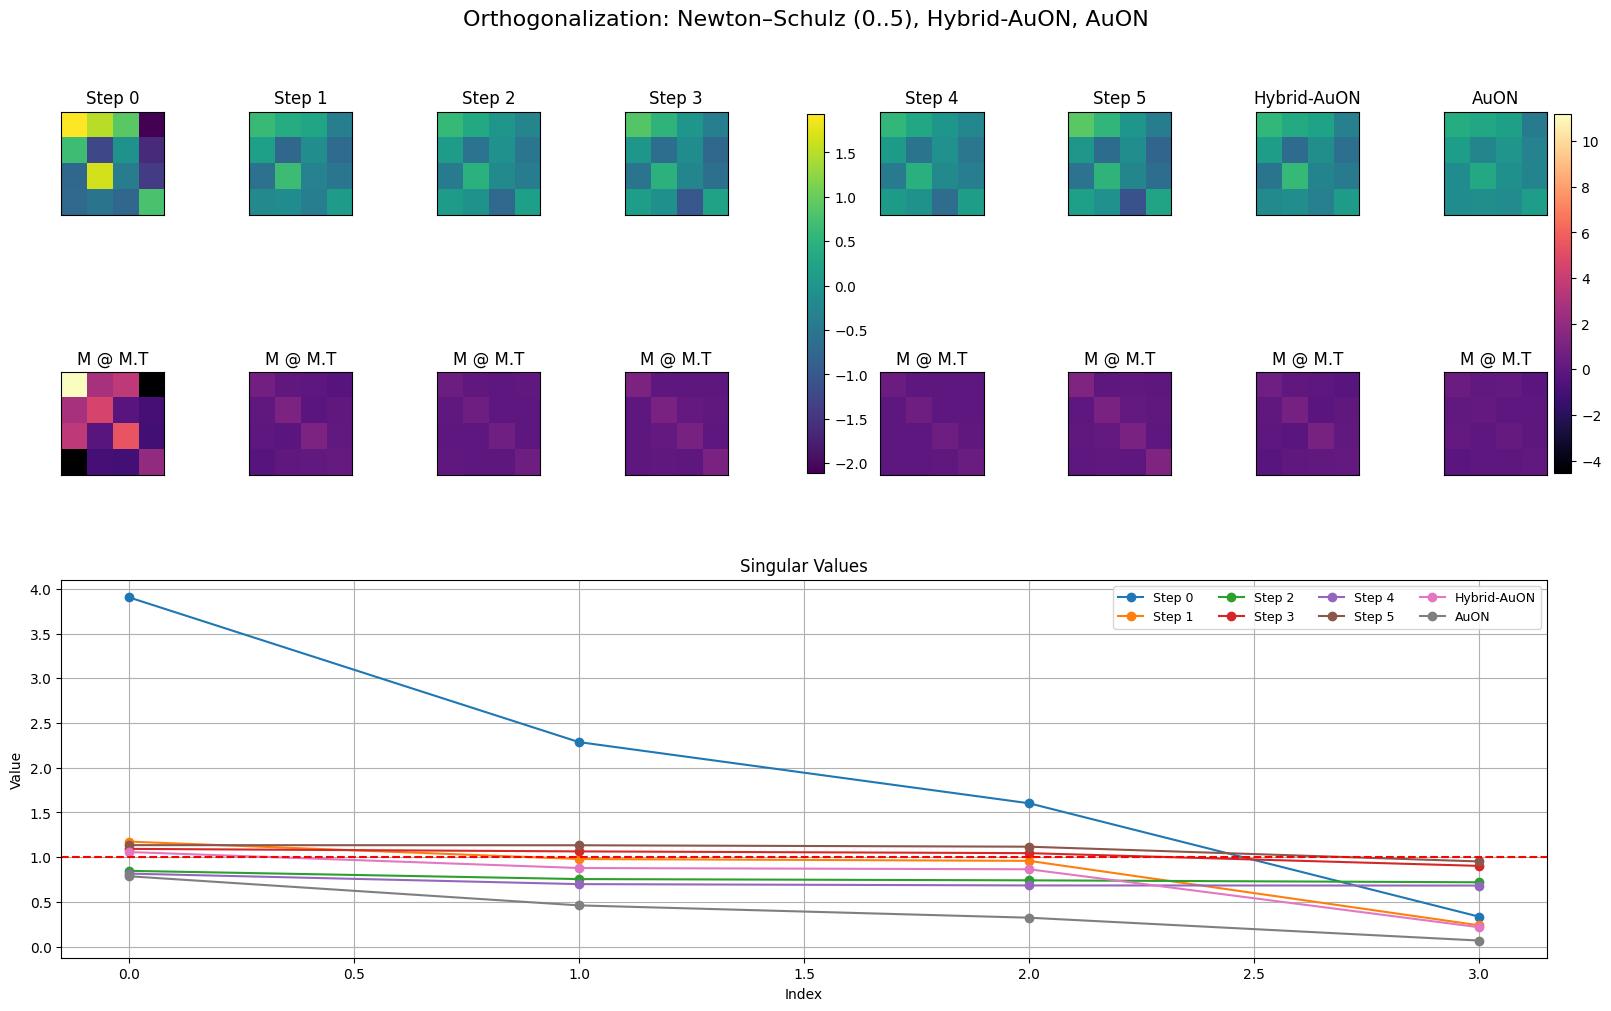
\includegraphics[width=1.0\linewidth]{all2.png}
   \caption{Visualization of the Newton–Schultz process (0.5) over 5 iterations, compared with AuON and Hybrid-AuON. 
The heatmaps (top) show progressive orthogonalization, with $M M^\top$ converging from a scattered structure (Step 0) to an identity-like diagonal (Step 5). 
The singular value plot (bottom) illustrates rapid convergence toward $1.0$, confirming orthogonalization.}
    \label{fig:training_curves}
    \vspace*{\fill}
\end{figure}
By orthogonalizing an update matrix, we effectively discard the scaling information encoded in the singular values and modify each direction to enforce perpendicularity, putting all the  update length into unit vectors(unit length) but different directions. In this sense, the resulting update behaves as a  "unit-norm"  update in the spectral domain, emphasizing the geometric structure of the optimization landscape rather than the raw magnitude of the gradients. In simple words, Orthogonalization effectively increases the scale of other “rare directions” which have small magnitude in the update but are nevertheless important for learning. Such a perspective highlights how orthogonalization can prioritize exploration across all relevant directions, potentially mitigating the dominance of a few high-energy directions and facilitating more balanced learning dynamics \parencite{zhang2025adagradmeetsmuonadaptive}. Orthogonalized updates can be interpreted as spectral descent directions, which helped to ensure updates explore all directions evenly, which is crucial for generalization and representation learning.

\parencite{tuddenham2022orthogonalisinggradientsspeedneural} proposed an approach for neural network optimization in which the gradient is first orthogonalized via singular value decomposition (SVD), followed by the application of momentum, and then the resulting momentum term is used as the update. They refer to this method as Orthogonal-SGDM. In their experiments, they observed that, even in their best-performing configuration, Orthogonal-SGDM was outperformed by a well-tuned standard SGD with momentum due to applying momentum after strict orthogonalization, as Orthogonal-SGDM essentially damages the momentum mechanism by orthogonalizing gradients before momentum accumulation, preventing momentum from effectively reducing variance and maintaining beneficial directional information and strict orthogonality thereby erases singular-value magnitudes and overconstrains the step, meaning it over-normalizes the update by collapsing its singular-value structure to an isometry, effectively turning the step into a spectral‑norm–constrained, normalized move that discards useful magnitude information. This wipes out all correlations between update directions. Makeing all the updates into unit length may be problematic as it may increase harmful alignment  . Recent advances, as such as Muon \parencite{jordan2024muon}, improve efficiency and performance by producing a semi-orthogonal matrix using Newton–Schulz iterations rather than a full orthogonal matrix using SVD and reordering the momentum update before the semi-orthogonalization, thereby reducing the complexity to \(O(n^2)\). But the computation cost of Newton-Schulz is still \( O(n^2) \).


In this paper, we focus on developing an alternative approach to bound the updates with a high condition number under  unit norm  . Our goal is -how to achieve an impressive performance at O(n) time complexity, meaning without compromising efficiency and speed. 
We empirically find that  normalization followed by a hyperbolic function(cosh) scale magnitude yields promising results 


%--------------------related work-------------------
% ---------------- Preliminaries ----------------
\section{Preliminaries}

\subsection{orthogonalization}





By orthogonalizing an update matrix 
$G \in \mathbb{R}^{m \times n}$ 
with singular value decomposition 
\[
G = U \Sigma V^{\top},
\]
The update is replaced by its orthogonal polar factor
\[
Q := U V^{\top}.
\]

This satisfies
\[
Q^{\top}Q = I_n \quad \text{when } m \geq n,
\qquad
QQ^{\top} = I_m \quad \text{when } m \leq n,
\]
thereby discarding the scaling information carried by the singular values 
$\Sigma$ while preserving the directional subspaces encoded by the left and right singular vectors $U$ and $V$.

In this sense, the resulting update behaves as unit-norm in the spectral domain—
\[
\|Q\|_{2} = 1
\]
with a flat singular spectrum—emphasizing the geometric structure of the optimization landscape rather than the raw gradient magnitudes.

Intuitively, this equalizes per-direction gain: directions that originally had small singular values (“rare directions”) are relatively amplified while dominant directions are relatively attenuated, promoting exploration across all relevant directions and mitigating the dominance of a few high-energy modes. 

In practice, orientation and step size can be decoupled by using 
\[
\alpha Q,
\qquad 
\alpha = \frac{\|G\|_{F}}{\sqrt{\mathrm{rank}(G)}},
\]
so that scale is controlled externally while orthogonalization enforces well-conditioned, balanced updates—yielding more stable and equitable learning dynamics compared to conventional gradient-descent steps.

\subsection{semi-orthogonalization}
Given $G \in \mathbb{R}^{m \times n}$ with singular value decomposition
\[
G = U \Sigma V^{\top},
\]
strict orthogonalization replaces $G$ by its polar/Stiefel projection
\[
Q := U V^{\top},
\]
collapsing the singular spectrum to $\sigma_i(Q) = 1$ on the update subspace and making $Q$ an isometry with
\[
\|Q\|_{2} = 1, 
\qquad 
Q^{\top} Q = I_n \; \; (\text{or } \; QQ^{\top} = I_m),
\]
i.e., the Frobenius-nearest semi-orthogonal matrix that removes the amplitude information in $\Sigma$.\parencite{article2}

In the singular basis,
\[
G^{\top} G = V \Sigma^{2} V^{\top}
\]
becomes
\[
Q^{\top} Q = I,
\qquad
QQ^{\top} = U I U^{\top} = \Pi_{\mathrm{col}(G)},
\]
turning the step into a spectral-norm–bounded move that can discard curvature-aligned anisotropy.  

Geometrically, for Muon’s RMS-to-RMS operator norm, we have
\[
Q \in \arg\max_{\|X\|_{\mathrm{RMS}\to\mathrm{RMS}} \leq 1} \langle X, G \rangle,
\]
which is the linear minimization oracle (LMO) of a conditional-gradient step. Hence the singular values are flattened; by contrast, on the standard spectral-norm ball, the LMO yields the rank-1 solution $u_{1} v_{1}^{\top}$.\parencite{lee2021_vonneumann}

To avoid overconstraint, semi-orthogonal schemes such as Muon orthogonalize only the momentum $M_t$ to
\[
Q_t = \mathrm{polar}(M_t),
\]
and decouple scale via an RMS-to-RMS factor $\alpha$, giving
\[
W_{t+1} = (1 - \eta_t \lambda) W_t + \eta_t \, \alpha \, Q_t.
\]
In practice, $Q_t Q_t^{\top}$ is computed efficiently via a low-order Newton–Schulz iteration, and $\alpha$ is chosen to match update RMS across shapes, enabling stability and learning-rate transfer. Semi‑orthogonalization stabilizes training by bounding spectral energy and equalizing directional gains, preventing overshoot along sharp curvature, reducing oscillations, and enabling larger learning rates by decoupling orientation from scale\parencite{liu2025muonscalablellmtraining}

\subsection{Orthogonalized Momentum as a Spectral Trust-Region Method}

Recent advances demonstrate that orthogonalized momentum in deep learning optimizers, particularly the Muon optimizer, admits a principled interpretation as the solution to a non-Euclidean trust-region subproblem under the spectral norm constraint~\parencite{kovalev2025understandinggradientorthogonalizationdeep}. The core update rule can be formulated as
\[
X_{k+1} = X_k - \eta O_k,
\quad 
O_k = \mathrm{Orth}\!\left(\nabla F(X_k)\right),
\]
where $\mathrm{Orth}(\cdot)$ denotes the SVD-based orthogonalization operator that computes
\[
M = U \Sigma V^\top 
\quad \Longrightarrow \quad 
\mathrm{Orth}(M) = U V^\top,
\]
yielding the steepest descent direction under the spectral norm metric.

\textbf{Momentum Integration}
The momentum component follows the exponential moving average
\[
m_{k+1} = (1-\alpha)m_k + \alpha \, g(x_k;\xi_k),
\]
where $g(x_k;\xi_k)$ represents an unbiased stochastic gradient estimate. The orthogonalized update then solves the trust-region subproblem
\[
x_{k+1} 
= \arg\min_{x} 
\Big\{ \langle \mathrm{Orth}(m_{k+1}), \, x \rangle 
: \, \|x - x_k\|_2 \leq \eta \Big\}.
\]
This formulation explicitly constrains parameter updates within a trust region while ensuring the search direction maintains unit spectral norm.

\textbf{Theoretical Advantages}
The orthogonalization-first approach provides superior variance reduction compared to alternative momentum--orthogonalization orderings. By applying orthogonalization to the momentum vector before the parameter update, the method preserves the accumulated directional information while eliminating scale-dependent instabilities. This design choice demonstrates both theoretical guarantees for convergence under non-convex objectives and empirical improvements in training stability across diverse architectures \parencite{liu2025muonscalablellmtraining}.

% ---------------- Methods ----------------
\section{Methods}
We hypothesize that forcing all update directions to unit length can be problematic, as not all directions contribute equally to optimization progress—some may be harmful (having a negative impact) or irrelevant to loss reduction. Our goal is to develop an alternative method that removes the harmful directions or alignments and  preserves the beneficial properties of near semi-orthogonalization while selectively scaling directions under unit-norm : decrease the  scales  of  "rare updates directions" than the dominant update directions and keep them all under a unit-norm trust region, meaning prioritizing directions with favorable conditioning that correspond to well-conditioned subspaces of the loss landscape under a spectral-norm trust-region.One solution is to apply a temperature-scaled softmax update matrix, followed by L2 renormalization, to bound the step under a trust-region. But computing softmax may be problematic as it comes with its own bottleneck, and it does not preserve the semi-orthogonal property that is needed for an optimizer like Muon .
We empirically find out that the  normalization with hyperbolic functions (cosh ) help us achieve spectral-norm trust-region \parencite{kovalev2025understandinggradientorthogonalizationdeep} and helps us preserve the near semi-orthogonal properties that is more stable and equitable learning dynamics compared to conventional gradient-descent steps, and stabilizes training by bounding spectral  energy into a unit vector and equalizing directional gains, preventing overshoot along sharp curvature, reducing oscillations, and
enabling larger learning rates by decoupling orientation from scale\parencite{Peletier_2023}

\subsection{Nonlinear reshaping via hyperbolic cosine RMS scaling}
Our main goal is to keep all the updated directions under unit spectral norm and remove the hermful directions. We empirically find out  the updated matrix divided by the scale factor of the RMS magnitude of cosh() helps us bound the dominant update directions which have a high condition number under  unit spectral norm, and helps us to preserve the near semi-orthogonal-like properties.By doing this, we remove the harmful alignment and stabilize the updates and equitable learning dynamics. The overall equation is 


\[ X = \frac{G}{\|G\| + 10^{-7}} \] \[ \text{update} = X \] \[ x = \cosh(\text{update}) \] \[ \text{rms} = \sqrt{\frac{1}{N} \sum_{i=1}^{N} x_i^2} \] \[ G = \frac{\text{update}}{\text{rms} + 10^{-8}} \]


where

\[
\cosh(z) = \frac{e^z + e^{-z}}{2}
\]

For large values of \( |z| \), \(\cosh(z)\) grows exponentially, while for small values of \(z\),
\[
\cosh(z) \approx 1 + \frac{z^2}{2}.
\]

Thus, \(\cosh\) magnifies meaningful deviations while remaining symmetric and smooth.

This encourages a spread of activations (diversity) without enforcing strict  orthogo- \indent nality \parencite{Peletier_2023} and X is the updated momentum vector direction 

\noindent\textbf{Effect of the Hyperbolic Cosine RMS Magnitude.}\\
Define \(\mathrm{rms} := \|\cosh(\mathrm{update})\|_{F}/\sqrt{N}\), where \(\cosh\) is applied \emph{only} to compute a global, tail‑sensitive scale \parencite{article}. Because \(\cosh\) is even and rapidly increasing in \(|x|\), heavy tails inflate \(\mathrm{rms}\), which reduces the overall step size when forming \(U := \mathrm{update}/(\mathrm{rms}+10^{-8})\). Crucially, \(\cosh\) is not applied to the propagated vector: \(U\) is a uniform rescaling of \(\mathrm{update}\), so the signs and all relative component ratios of \(\mathrm{update}\) are preserved in \(U\). This yields scale invariance with tail‑aware damping, without introducing per‑coordinate reweighting in the final update.

\medskip
\noindent\textbf{Layman’s terms.}
First, fix the raw step’s size; then gauge how “spiky” it is using \(\cosh\); finally, shrink the whole step more if it looks spiky. The direction and internal proportions of the step stay the same.

\medskip
\noindent\textbf{Near–Semi–Orthogonality.}

\noindent\textbf{Exact orthogonality.}
A matrix \(W \in \mathbb{R}^{m \times n}\) is orthogonal (semi‑orthogonal if \(m \neq n\)) when
\[
W^\top W = I_n \quad \text{or} \quad W W^\top = I_m ,
\]
which preserves Euclidean inner products and hence norms and angles exactly.

\medskip
\noindent\textbf{Method (equations).}
Let \(G \in \mathbb{R}^{m \times n}\) be a gradient/update and \(N := mn\). Define
\[
\mathrm{update} := \frac{G}{\|G\|_{F} + 10^{-7}}, 
\qquad
\mathrm{rms} := \frac{\big\| \cosh(\mathrm{update}) \big\|_{F}}{\sqrt{N}},
\qquad
U := \frac{\mathrm{update}}{\mathrm{rms} + 10^{-8}}.
\]
Equivalently, \(U = X/(r+\varepsilon)\) with \(X=\mathrm{update}\), \(r=\mathrm{rms}\), \(\varepsilon=10^{-8}\).

\medskip
\noindent\textbf{Immediate implications.}
\begin{itemize}
\item \emph{Scale invariance.} For any \(c>0\), replacing \(G\) by \(cG\) leaves \(\mathrm{update}\) (and thus \(U\)) unchanged up to \(\varepsilon\)-terms.
\item \emph{Tail‑aware global scaling.} Heavy tails inflate \(\mathrm{rms}\) via \(\cosh\), reducing the global magnitude of \(U\) when the update is spiky.
\item \emph{No per‑component reweighting.} \(U\) is a uniform rescaling of \(\mathrm{update}\); signs and relative component ratios of \(\mathrm{update}\) are preserved in \(U\).
\end{itemize}

\medskip
\noindent\textbf{Norms and “balanced sphere.”}
This construction does not enforce unit RMS for \(U\). Indeed,
\begin{align}
\|\mathrm{update}\|_{F} \approx 1,\qquad\\
\|U\|_{F} = \frac{\|\mathrm{update}\|_{F}}{\mathrm{rms} + 10^{-8}} \approx \frac{1}{\mathrm{rms} + 10^{-8}},\\
\qquad\mathrm{RMS}(U) = \frac{\|U\|_{F}}{\sqrt{N}} \approx \frac{1}{\sqrt{N}\,(\mathrm{rms}+10^{-8})}\ \end{align}
Thus, there is no unit‑L2 or unit‑RMS constraint on \(U\); the overall step length decreases as the tail‑sensitive scalar \(\mathrm{rms}\) increases.

\medskip
\noindent\textbf{Relation to near semi‑orthogonality.}
Let 
\[
M := U^\top U \in \mathbb{R}^{n \times n}.
\]
By the Frobenius–trace identity,
\[
\operatorname{tr}(M) = \|U\|_F^2,
\]
and
\[
\alpha := \frac{1}{n} \operatorname{tr}(M),
\]
which equals the average column $\ell_2$ norm squared.  

However, under the mapping above, $\operatorname{tr}(M)$ is determined by $\mathrm{rms}$ and is not generally $N = mn$ unless an extra unit-RMS rescale is applied to $U$.  

Off-diagonal correlations 
\[
M_{ij} = \langle U_{:i}, U_{:j} \rangle
\]
are not explicitly zeroed by this mapping, so it promotes scale invariance and approximate isotropy rather than exact semi-orthogonality.
\begin{itemize}
\item \emph{Cross‑correlations.} Off‑diagonals of \(M\) are scaled copies of those in \(\mathrm{update}^\top \mathrm{update}\); they are not explicitly suppressed.
\item \emph{Isotropy.} This mapping alone does not drive \(M\) toward \(\alpha I_n\). Achieving near semi‑orthogonality typically requires an additional correlation‑reducing step (e.g., per‑column RMS normalization, light whitening, or a spectral penalty \(\|U^\top U - \alpha I\|_F^2\) with \(\alpha=\tfrac{1}{n}\operatorname{tr}(U^\top U)\)). see Appendix A for more information
\end{itemize}

\noindent\textbf{Practical implication.}\\
The update is scale‑invariant and tail‑aware: heavy tails trigger stronger global shrinkage via \(\mathrm{rms}\), helping prevent blow‑ups while preserving the direction and internal proportions of the step. When approximate isotropy or near semi‑orthogonality is desired, pair this normalization with a lightweight correlation‑suppressing operation.




⁡\subsection{Hybrid Approach}
\begin{figure}[!htb]
    \vspace*{\fill}
    \centering
    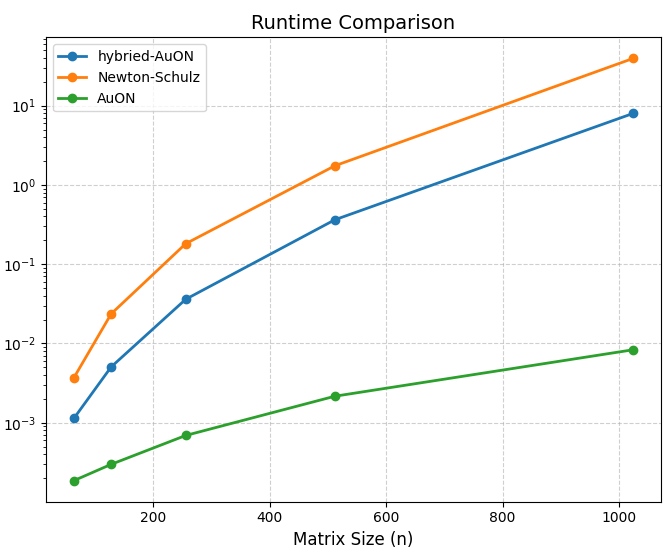
\includegraphics[width=0.5\linewidth]{auon2.png}
   \caption{comparison of computation efficiency of different methods on (nxn) ramdom matrices}
    \label{fig:training_curves}
    \vspace*{\fill}
\end{figure}

The hybrid approach include only one iteration of Newton-Schulz and Nonlinear reshaping via hyperbolic cosine RMS scaling. this helps use improve the performance only using one iteration.


\[
A = X X^\top
\]

\[
B = bA + cA^2
\]

\[
X \leftarrow aX + BX
\]

\[
G_{\text{new}} = \frac{\text{update}}{\mathrm{rms} + \delta},
\quad 
\text{with } \text{update} = X,
\quad 
\mathrm{rms} = \frac{1}{N} \| \cosh(X) \|_F^2.
\]
it helps us to achieve  near semi-orthogonality   and bound the updates under  spectral-norm trust-region with comparable less computation than Newton-Schulz 5 times iteration in Muon and can achive impressive  performance compare to Adamw and Muon

% ---------------- Experiments ----------------
\section{Experiments}
\subsection{Language Modeling}
We evaluate our approach using  4X L4 GPU   on  the \textbf{SmolLM-Corpus} dataset\parencite{benallal2024smollmcorpus} , consisting of 500k tokens. 
The underlying model is a nanoGPT\parencite{Karpathy2022} with FlashAttention-2\parencite{dao2023flashattention2fasterattentionbetter} rotary position embeddings (RoPE)\parencite{su2023roformerenhancedtransformerrotary}, RMSNorm \parencite{huang2019rmsnorm}, and SwiGLU activations \parencite{shazeer2020gluvariantsimprovetransformer}. 
For the \textbf{Small configuration}, we use a hidden size of 512, 6 layers, 8 attention heads, and a feed-forward dimension of 1536. 
Training is conducted for 6000 steps with a global batch size of 128. 
We compare \textsc{AuON}, AdamW \parencite{loshchilov2019decoupledweightdecayregularization}, Hybrid-AuON, and MuON under similar training conditions, with learning rates tuned separately: 
$\eta_{\text{adamw}} = 0.003$, $\eta_{\text{auon}} = 0.055$. and $\eta_{\text{muon}} = 0.01$. \parencite{rosic2025muon}

\begin{table}[h] 
\centering
\caption{Training Results on Tiny (Run 1). All optimizers are trained under identical settings.}
\label{tab:tiny_run1}
\begin{tabular}{lcccccc}
\hline
\textbf{Optimizer} & \textbf{Total Params} & \textbf{Opt. Params} & \textbf{Time (s)} & \textbf{Loss} & \textbf{Acc} & \textbf{PPL} \\
\hline
AuON         & 40,901,120 & 15,728,640 & 1919.2 & 0.4305 & 0.8667 & 1.54 \\
AdamW        & 40,901,120 & 25,172,480 & 1918.9 & 0.0686 & 0.9846 & 1.07 \\
Hybrid-AuON  & 40,901,120 & 15,728,640 & 2285.4 & 0.0422 & 0.9908 & 1.04 \\
MuON         & 40,901,120 & 15,728,640 & 2303.6 & 0.0375 & 0.9919 & 1.04 \\
\hline
\end{tabular}
\end{table}

\subsection{vision task}


We evaluated \textbf{AdamW} and the proposed \textbf{Auon optimizer} on the CIFAR-10 dataset under a reduced-scale training protocol. A random seed (42) ensured reproducibility. The dataset was split into \textbf{15,000 training}, \textbf{1,500 validation}, and \textbf{5,000 test} samples. Data loading used a batch size of 32 with standard preprocessing.

\noindent \textbf{Training configuration:} 100 epochs, learning rate = $1\times 10^{-3}$, Muon LR = 0.055, weight decay = $1\times 10^{-4}$, momentum $(\beta_{1}, \beta_{2}) = (0.9, 0.99)$. The network contained 19.90M parameters.

\noindent \textbf{Results (Test Accuracy):}
\begin{itemize}
    \item AdamW: 76.0\%
    \item Auon: 73.3\%
    \item $\Delta = -2.7$ percentage points
\end{itemize}

AdamW outperformed Auon in this small-scale setting, though performance may be affected by the limited dataset size and training duration.
\begin{figure}[!htb]
    \vspace*{\fill}
    \centering
    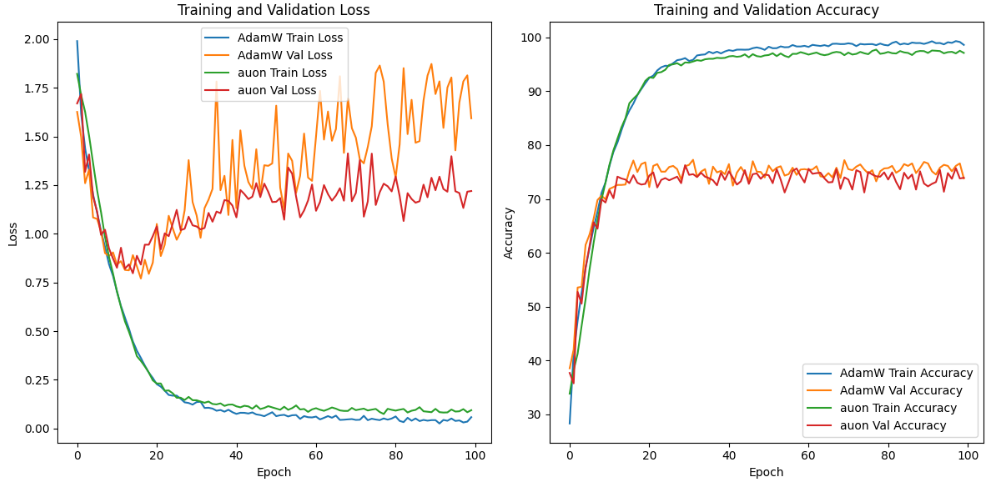
\includegraphics[width=1\linewidth]{scr.png}
   \caption{Training and validation curves on CIFAR-10 with AdamW and AuON optimizers. 
    (Left) Loss decreases steadily for AdamW, while AuON exhibits higher and more unstable loss. 
    (Right) Accuracy shows AdamW converging to $\sim$76\% while AuON plateaus around 73\%.}
    \label{fig:training_curves}
    \vspace*{\fill}
\end{figure}\\

But increasing the batch size from 32 to 128 can improve the performance
\noindent \textbf{Results (Test Accuracy):}
\begin{itemize}
    \item AdamW: 76.32\%
    \item Auon: 76.22\%
    \item $\Delta = -0.10$ percentage points
\end{itemize}


% ---------------- Conclusion ----------------
\section{Conclusion}
In this paper, we only focus on the linear time  Optimizer that has  unit-spectral-norm and other semi-orthogonal  properties that are needed for stabilized training  without the need for the proper semi-orthogonalization. Through our experiment, we suspect   that Auon and its Hybrid-variant may suffer from exploding attention logits\parencite{kimiteam2025kimik2openagentic} on Large parameter models, due to a lack of higher GUP resources; we cannot conduct such experiments. We can use qk-clipping as describe in \parencite{kimiteam2025kimik2openagentic} to reduce the effect. We empirically find out that increasing the model parameters   increases the AuON accuracy by up to 92 percent, and furthermore, on the downstream tasks. As future work, we plan to evaluate our approach on the NanoGPT speedrun using H100 GPUs, to assess its performance in a larger-scale, practical training setting.
% ---------------- References ----------------
\printbibliography



\end{document}

